\documentclass[journal,10pt]{IEEEtran}
\usepackage[utf8]{inputenc}
\usepackage[T1]{fontenc}
\usepackage{lmodern}
\usepackage{amsmath}
\usepackage{booktabs}
\usepackage{array}
\usepackage{multirow}
\usepackage{graphicx}
\usepackage{xcolor}
\usepackage{tikz}
\usetikzlibrary{arrows.meta,positioning,shapes.misc,calc,fit}
\usepackage{listings}
\usepackage{url}
\usepackage[hidelinks]{hyperref}
\usepackage{microtype}

\lstset{basicstyle=\ttfamily\footnotesize,columns=fullflexible,keepspaces=true,
        frame=single,framerule=0.3pt,xleftmargin=2pt,xrightmargin=2pt,breaklines=true}

\newcommand{\soc}{Small\_SoC}
\newcommand{\reg}[1]{\texttt{#1}}

\begin{document}

\title{\soc: Design, Verification and FPGA Implementation of a From-Scratch\\
RV32I Microcontroller System-on-Chip with an AXI-Lite Fabric\\and a JTAG Debug Port}

\author{Krishna~Gorai%
\thanks{K. Gorai is with the Indian Institute of Technology Mandi, India
(e-mail: kg05112001@gmail.com). Project repository:
\url{https://github.com/Krishna-Gorai/small-soc-riscv}.}}

\markboth{Project Report, September 2026}{Gorai: \soc\ -- an RV32I microcontroller SoC on the ZCU104}

\maketitle

\begin{abstract}
This report describes \soc, a complete microcontroller-class system-on-chip
written from scratch in synthesisable Verilog-2001 without any vendor
intellectual property. The system consists of a multicycle RV32I processor
core with the Zicsr extension and machine-mode trap handling, a hand-written
AMBA AXI4-Lite interconnect, a 32~KB block-RAM program memory, general-purpose
I/O, a UART, a timer with an interrupt line, and a JTAG debug port that can
halt the core, access every bus address and load a program without
rebuilding the bitstream. A C tool-chain (linker script, start-up code, trap
vector and board-support library) targets the SoC with an unmodified GNU
compiler. Correctness is established at four levels: the core passes all 41
applicable programs of the official \texttt{riscv-tests} rv32ui suite; two
application programs run as self-checking simulations; the debug port is
exercised end-to-end by a JTAG bus-functional model; and the placed-and-routed
netlist is simulated at gate level with the real board clock. On a Xilinx Zynq
UltraScale+ XCZU7EV (ZCU104 board) the SoC occupies 1\,710 look-up tables,
985 flip-flops and 8 block RAMs, meets timing at 100~MHz with 5.3~ns of slack,
and the debug port adds about 190 look-up tables. The report gives the
architecture, the working mechanism of every block, the verification
methodology and the implementation results, and records the design decisions
and the problems met along the way.
\end{abstract}

\begin{IEEEkeywords}
RISC-V, system-on-chip, AXI4-Lite, JTAG, boundary scan, FPGA, Verilog,
processor design, hardware verification.
\end{IEEEkeywords}

% =====================================================================
\section{Introduction}
% =====================================================================
A system-on-chip (SoC) is a processor together with the memory, the
interconnect and the peripherals it needs to run a program and to talk to the
outside world. Commercial SoCs are assembled from licensed blocks and vendor
generators, which hides the mechanisms a designer must understand to build,
verify and debug one. \soc\ is the opposite exercise: every block, from the
instruction decoder to the JTAG test-access port, is written by hand in plain
Verilog-2001, so that every line can be explained and every behaviour can be
traced to the RTL that produces it.

The design implements the 32-bit RISC-V base integer instruction set (RV32I)
\cite{riscv-unpriv} together with the control-and-status-register extension
(Zicsr) and the machine-mode subset of the privileged architecture
\cite{riscv-priv} that is needed for traps and interrupts. The core talks to
its memory and peripherals through the AMBA AXI4-Lite protocol \cite{axi},
the lightweight subset of AXI4 used for register-mapped devices. A debug
port, reached through the FPGA's own JTAG chain \cite{ieee1149}, lets a host
stop the core, inspect and modify memory and peripheral registers, and load
programs. The SoC is implemented on the Xilinx Zynq UltraScale+ ZCU104
evaluation board \cite{ug1267} and runs C programs produced by the unmodified
GNU tool-chain.

The report is organised as follows. Section~\ref{sec:motivation} states the
goals and the constraints they impose. Section~\ref{sec:background} recalls
the standards the design implements. Section~\ref{sec:arch} presents the
system architecture and the memory map. Sections~\ref{sec:core} to
\ref{sec:jtag} describe the working mechanism of the core, the bus, the
peripherals and the debug port. Section~\ref{sec:sw} covers the software
stack, Section~\ref{sec:verif} the verification methodology, and
Section~\ref{sec:impl} the FPGA implementation and its results.
Section~\ref{sec:lessons} records the problems encountered and how they were
resolved, and Section~\ref{sec:conclusion} concludes with future work.

% =====================================================================
\section{Motivation and Objectives}\label{sec:motivation}
% =====================================================================
The project has one primary goal and four derived requirements.

\textbf{Goal.} Produce a small but complete SoC that a single designer can
defend in full: no block may be a black box, and every claim about it must be
backed by a reproducible test.

\textbf{Correctness before performance.} The core is a multicycle machine
rather than a pipeline. A pipeline would raise instructions per cycle but
would add hazards, forwarding and flushing logic whose verification would
dominate the project. A multicycle controller has one instruction in flight
at a time; its correctness can be argued state by state and confirmed with
the standard instruction-set tests.

\textbf{Standard interfaces.} The bus is AXI4-Lite and the debug port is
reached through IEEE~1149.1 JTAG, so that the blocks can be understood, and
reused, by anyone who knows those standards, and so that the debug port works
with the board's existing USB-JTAG cable rather than needing a dedicated
header.

\textbf{Real software.} The SoC must run C code compiled by an unmodified GNU
compiler, which requires a linker script, start-up code and a trap vector
that match the hardware exactly.

\textbf{Evidence at every level.} Register-transfer-level (RTL) simulation
alone does not prove that a design works on silicon. The project therefore
also checks the placed-and-routed netlist by simulation and reports the
implementation numbers from the vendor tools.

% =====================================================================
\section{Background}\label{sec:background}
% =====================================================================
\subsection{RV32I, Zicsr and Machine Mode}
RV32I \cite{riscv-unpriv} has 32 general-purpose registers of 32 bits
(\reg{x0} is hard-wired to zero), a 32-bit program counter, and 40
instructions in six encoding formats (R, I, S, B, U, J). All instructions
are 32 bits wide and word-aligned. Loads and stores access bytes, half-words
and words; branches compare two registers; \reg{jal}/\reg{jalr} implement
calls and indirect jumps; \reg{lui}/\reg{auipc} build 32-bit constants and
PC-relative addresses.

Zicsr adds six instructions (\reg{csrrw}, \reg{csrrs}, \reg{csrrc} and their
immediate forms) that read and modify the control-and-status registers
(CSRs), a separate 4096-entry address space. The privileged architecture
\cite{riscv-priv} defines, for machine mode (M-mode), the CSRs that control
traps: \reg{mstatus} (global interrupt enable \reg{MIE} and its saved copy
\reg{MPIE}), \reg{mie}/\reg{mip} (per-source interrupt enable and pending
bits), \reg{mtvec} (trap vector), \reg{mepc} (return address),
\reg{mcause} (trap cause) and \reg{mscratch}. A trap saves the PC in
\reg{mepc}, records the cause, disables interrupts and jumps to \reg{mtvec};
the \reg{mret} instruction reverses this. \reg{ecall} and \reg{ebreak} raise
synchronous traps from software.

\subsection{AMBA AXI4-Lite}
AXI4-Lite \cite{axi} is a memory-mapped bus with five independent channels:
read address (AR), read data (R), write address (AW), write data (W) and
write response (B). Each channel carries a \reg{VALID} from its source and a
\reg{READY} from its sink; a transfer takes place on the clock edge where
both are high. A source must not withdraw \reg{VALID} once asserted until the
transfer completes, and must not make \reg{VALID} depend on \reg{READY}. All
transfers are single 32-bit words; writes carry a 4-bit byte strobe
(\reg{WSTRB}). Because the channels are independent, AW and W may arrive in
either order and a slave must accept both before responding on B.

\subsection{IEEE 1149.1 JTAG and Xilinx BSCANE2}
The JTAG test-access port (TAP) \cite{ieee1149} is a four-wire serial
interface (\reg{TCK}, \reg{TMS}, \reg{TDI}, \reg{TDO}) driven by a 16-state
controller. \reg{TMS} steers the controller between the instruction-register
(IR) and data-register (DR) scan paths; in the \emph{Shift} states one bit
enters on \reg{TDI} and one leaves on \reg{TDO} per \reg{TCK}; the
\emph{Capture} state loads a register before shifting and the \emph{Update}
state commits it afterwards. Every device has a \reg{BYPASS} and an
\reg{IDCODE} instruction; vendors add \emph{user} instructions that connect
the DR path to user logic. On Xilinx UltraScale+ devices the \reg{BSCANE2}
primitive \cite{ug974} exposes one such user register: it presents
\reg{SEL}, \reg{CAPTURE}, \reg{SHIFT}, \reg{UPDATE}, \reg{TCK}, \reg{TDI} to
fabric logic and takes \reg{TDO} back, so a design can hang its own serial
register off the device's JTAG chain without any package pins.

% =====================================================================
\section{System Architecture}\label{sec:arch}
% =====================================================================
Fig.~\ref{fig:block} shows the SoC. One RISC-V core and one JTAG debug
master share a single AXI4-Lite fabric through a two-master arbiter; the
interconnect behind it decodes four slaves. The timer's interrupt line goes
back to the core; the debug port's halt and reset lines go to the core as
well. The whole design runs on one clock (\reg{clk}, 100~MHz on the board)
and one active-low asynchronous reset (\reg{rst\_n}), except for the debug
register, which is clocked by JTAG \reg{TCK} and crosses into the \reg{clk}
domain through synchronisers (Section~\ref{sec:jtag}).

\begin{figure}[t]
\centering
\resizebox{\columnwidth}{!}{%
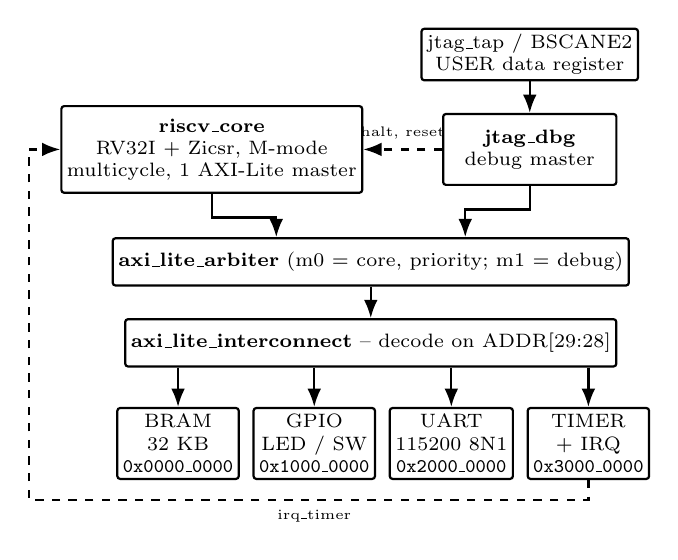
\begin{tikzpicture}[
  font=\scriptsize,
  blk/.style={draw,rounded corners=1pt,minimum height=6mm,inner sep=2pt,align=center},
  >=Latex, thick]
  \node[blk,minimum width=26mm,minimum height=11mm] (core) at (0,0)
    {\textbf{riscv\_core}\\RV32I + Zicsr, M-mode\\multicycle, 1 AXI-Lite master};
  \node[blk,minimum width=22mm,minimum height=9mm,right=10mm of core] (dbg)
    {\textbf{jtag\_dbg}\\debug master};
  \node[blk,minimum width=24mm,above=4mm of dbg] (tap) {jtag\_tap / BSCANE2\\USER data register};
  \node[blk,minimum width=54mm,below=6mm of $(core.south)!0.5!(dbg.south)$] (arb)
    {\textbf{axi\_lite\_arbiter} (m0 = core, priority; m1 = debug)};
  \node[blk,minimum width=54mm,below=4mm of arb] (xbar)
    {\textbf{axi\_lite\_interconnect} -- decode on ADDR[29:28]};
  \node[blk,minimum width=12mm,minimum height=9mm,below=5mm of xbar.south west,anchor=north west,xshift=-1mm] (bram)
    {BRAM\\32 KB\\\reg{0x0000\_0000}};
  \node[blk,minimum width=12mm,minimum height=9mm,right=1.6mm of bram] (gpio)
    {GPIO\\LED / SW\\\reg{0x1000\_0000}};
  \node[blk,minimum width=12mm,minimum height=9mm,right=1.6mm of gpio] (uart)
    {UART\\115200 8N1\\\reg{0x2000\_0000}};
  \node[blk,minimum width=12mm,minimum height=9mm,right=1.6mm of uart] (tmr)
    {TIMER\\+ IRQ\\\reg{0x3000\_0000}};
  \draw[->] (core.south) -- ++(0,-3mm) -| ($(arb.north)+(-12mm,0)$);
  \draw[->] (dbg.south) -- ++(0,-3mm) -| ($(arb.north)+(12mm,0)$);
  \draw[->] (tap) -- (dbg);
  \draw[->] (arb) -- (xbar);
  \foreach \s in {bram,gpio,uart,tmr} { \draw[->] (xbar.south -| \s.north) -- (\s.north); }
  \draw[->,dashed] (tmr.south) -- ++(0,-2.5mm) -| ($(core.west)+(-4mm,0)$) -- (core.west);
  \node[font=\tiny,below] at ($(gpio.south)+(0,-2.5mm)$) {irq\_timer};
  \draw[->,dashed] (dbg.west) -- (core.east) node[midway,above,font=\tiny] {halt, reset};
\end{tikzpicture}}
\caption{Top level of \soc. Solid arrows are AXI4-Lite master-to-slave connections; dashed arrows are side-band control.}
\label{fig:block}
\end{figure}

\subsection{Memory Map}
The interconnect decodes address bits [29:28], which gives each slave a
256~MB window; each slave decodes bits [3:2] for its own registers and
ignores the rest. Table~\ref{tab:memmap} lists the map. Addresses inside a
window that a slave does not implement alias onto its registers; there is no
decode-error response, a simplification that is acceptable in a closed SoC
where all software is trusted.

\begin{table}[t]
\caption{Memory map and register definitions}
\label{tab:memmap}
\centering
\footnotesize
\begin{tabular}{@{}llp{4.6cm}@{}}
\toprule
Base & Block & Registers (offset: name, access) \\
\midrule
\reg{0x0000\_0000} & BRAM & 32 KB, byte-writable; code, data, stack; initialised from \reg{program.hex} in the bitstream \\
\reg{0x1000\_0000} & GPIO & \reg{+0} OUT (RW, LEDs); \reg{+4} IN (RO, switches and buttons) \\
\reg{0x2000\_0000} & UART & \reg{+0} TX (W: send byte; R: last byte); \reg{+4} RX (R, clears \reg{rx\_valid}); \reg{+8} STATUS \{bit1 \reg{rx\_valid}, bit0 \reg{tx\_busy}\} \\
\reg{0x3000\_0000} & Timer & \reg{+0} COUNT (RO); \reg{+4} COMPARE (RW); \reg{+8} CTRL \{bit1 \reg{irq\_en}, bit0 \reg{enable}\}; \reg{+C} STATUS \{bit0 \reg{pending}, write 1 to clear\} \\
\bottomrule
\end{tabular}
\end{table}

\subsection{Clocking and Reset}
Inside \reg{soc\_top} the board reset is passed through a two-flip-flop
synchroniser whose output, \reg{rst\_n}, is the asynchronous reset of every
block. The core receives \reg{rst\_n} ANDed with the inverse of the debug
port's core-reset request, so a debugger can reset the processor alone while
the peripherals, the memory contents and the debug logic keep their state.
The ZCU104 wrapper (Section~\ref{sec:impl}) derives the 100~MHz clock from
the board's 300~MHz differential oscillator with a single \reg{BUFGCE\_DIV}
primitive dividing by three; there is no MMCM, so no lock signal has to be
handled and no clocking IP has to be regenerated.

% =====================================================================
\section{Processor Core}\label{sec:core}
% =====================================================================
\subsection{Control: a Six-State Multicycle Machine}
The core executes one instruction at a time under the controller of
Fig.~\ref{fig:fsm}. \reg{IF\_ADDR} issues the fetch address on the AR
channel; \reg{IF\_DATA} waits for the instruction on the R channel and
latches it into \reg{instr\_reg}; \reg{EXEC} evaluates the instruction;
loads and stores pass through \reg{MEM\_ADDR} and \reg{MEM\_DATA} for the
data-side bus transaction; \reg{WB} writes the destination register, updates
the program counter and resolves traps. Table~\ref{tab:cycles} gives the
cost per instruction class with the zero-wait-state slaves of this SoC; the
run-time counters \reg{mcycle} and \reg{minstret} confirm an average of
about 5.6 cycles per instruction on the demonstration programs.

\begin{figure}[t]
\centering
\resizebox{\columnwidth}{!}{%
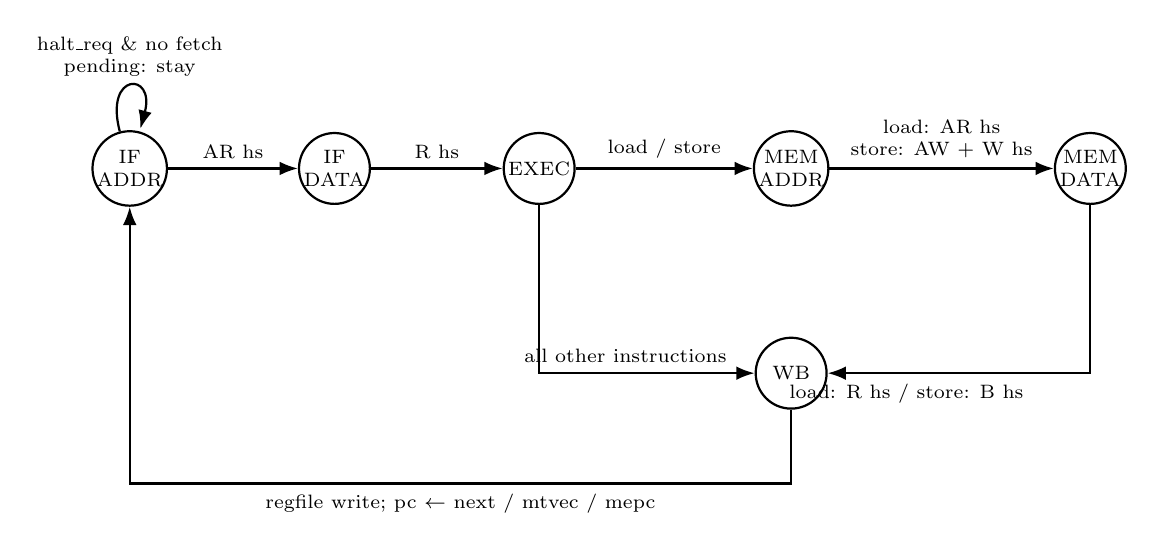
\begin{tikzpicture}[font=\scriptsize,>=Latex,thick,
  st/.style={draw,circle,minimum size=9mm,inner sep=0pt,align=center}]
  \node[st] (ifa) at (0,0) {IF\\ADDR};
  \node[st] (ifd) at (2.6,0) {IF\\DATA};
  \node[st] (ex)  at (5.2,0) {EXEC};
  \node[st] (ma)  at (8.4,0) {MEM\\ADDR};
  \node[st] (md)  at (12.2,0) {MEM\\DATA};
  \node[st] (wb)  at (8.4,-2.6) {WB};
  \draw[->] (ifa) -- node[above]{AR hs} (ifd);
  \draw[->] (ifd) -- node[above]{R hs} (ex);
  \draw[->] (ex)  -- node[above]{load / store} (ma);
  \draw[->] (ma)  -- node[above,align=center]{load: AR hs\\store: AW + W hs} (md);
  \draw[->] (md)  |- node[pos=0.85,below]{load: R hs / store: B hs} (wb);
  \draw[->] (ex)  |- node[pos=0.7,above]{all other instructions} (wb);
  \draw[->] (wb)  -- ++(0,-1.4) -| node[pos=0.25,below]{regfile write; pc $\leftarrow$ next / mtvec / mepc} (ifa);
  \draw[->] (ifa) edge[loop above] node[align=center]{halt\_req \& no fetch\\pending: stay} (ifa);
\end{tikzpicture}}
\caption{Core controller. ``hs'' denotes an AXI handshake (\reg{VALID}\,$\wedge$\,\reg{READY}). A debug halt request is honoured in \reg{IF\_ADDR} before a fetch is issued.}
\label{fig:fsm}
\end{figure}

\begin{table}[t]
\caption{Cycles per instruction class}
\label{tab:cycles}
\centering
\footnotesize
\begin{tabular}{@{}p{3.8cm}cp{3.1cm}@{}}
\toprule
Class & Cycles & States visited \\
\midrule
ALU (R/I), LUI, AUIPC, branch, JAL, JALR, CSR, system & 5 & IF\_ADDR(2), IF\_DATA, EXEC, WB \\
Load, store & 7 & + MEM\_ADDR, MEM\_DATA \\
\bottomrule
\end{tabular}
\end{table}

\subsection{Datapath}
All decode is combinational from \reg{instr\_reg}: the opcode, register
indices and the five immediate formats are wires. The ALU is a 32-bit
combinational block with eleven operations (add, subtract, and, or, xor,
three shifts, two compares and a pass-through used by \reg{lui}); its
operands are selected by instruction class (\reg{pc} for \reg{auipc}/\reg{jal},
zero for \reg{lui}, \reg{rs1} otherwise; \reg{rs2} or the appropriate
immediate). A separate comparator evaluates the six branch conditions. The
next PC is chosen among \reg{pc+4}, the branch target, the \reg{jal} target
and the \reg{jalr} target (with bit~0 cleared as the specification requires).

The register file is \reg{regs[1:31]}; \reg{x0} is a multiplexer that returns
zero rather than storage. Reads are combinational; the write port is
registered (\reg{rd\_we}, \reg{rd\_waddr}, \reg{rd\_wdata}) so the write
lands in the cycle after \reg{WB}, which is always before the next
instruction reaches \reg{EXEC}. Vivado maps it to 40 LUT-RAMs.

\subsection{Loads and Stores}
The core issues only word-aligned bus transactions. For a load, the word
returned on the R channel is steered and extended according to \reg{funct3}
(byte, half-word or word; signed or zero-extended) and the two low address
bits latched in \reg{mem\_addr\_reg}. For a store, the data is placed in the
correct byte lanes and \reg{WSTRB} is set to the matching pattern, so a
\reg{sb} to address \reg{0x...3} drives \reg{WDATA[31:24]} with
\reg{WSTRB=4'b1000}. Naturally aligned accesses are therefore correct for all
five load and three store instructions; misaligned accesses are not
supported and raise no exception, which is why the \reg{ma\_data} test is
excluded from the regression.

\subsection{Bus Master Behaviour}
The core's AXI outputs are registered. In \reg{IF\_ADDR} it raises
\reg{ARVALID} with the PC on \reg{ARADDR} and holds both until
\reg{ARREADY}; it then raises \reg{RREADY} and holds \reg{ARADDR} stable
until the data arrives. For a store it raises \reg{AWVALID} and
\reg{WVALID} together and tracks their acceptance separately (the
\reg{aw\_done}/\reg{w\_done} flags), asserting \reg{BREADY} only when both
have completed. Holding the address stable for the whole transaction is what
lets the interconnect route the response channels by address alone.

\subsection{Control and Status Registers}
Table~\ref{tab:csr} lists the implemented CSRs. \reg{csr\_rdata} is a
combinational read multiplexer; the write value is computed from the
operation (\reg{csrrw} writes the operand, \reg{csrrs} ORs it in,
\reg{csrrc} clears it) using either \reg{rs1} or the 5-bit immediate. A
\reg{csrrs}/\reg{csrrc} with \reg{rs1=x0} is a pure read, as the
specification requires. \reg{mcycle} increments every clock; \reg{minstret}
increments in \reg{WB}. Unknown CSRs read as zero and ignore writes.

\begin{table}[t]
\caption{Implemented control and status registers}
\label{tab:csr}
\centering
\scriptsize
\begin{tabular}{@{}p{2.4cm}p{2.0cm}p{3.4cm}@{}}
\toprule
CSR & Address & Implemented fields \\
\midrule
\reg{mstatus}  & \reg{0x300} & MIE (bit 3), MPIE (bit 7) \\
\reg{misa}     & \reg{0x301} & read-only \reg{0x4000\_0100} (RV32I) \\
\reg{mie}      & \reg{0x304} & MTIE (bit 7) \\
\reg{mtvec}    & \reg{0x305} & base, direct mode \\
\reg{mscratch} & \reg{0x340} & 32 bits \\
\reg{mepc}     & \reg{0x341} & bits [31:2] \\
\reg{mcause}   & \reg{0x342} & 32 bits \\
\reg{mip}      & \reg{0x344} & MTIP (bit 7) = timer IRQ input, read-only \\
\reg{mcycle[h]}, \reg{cycle[h]} & \reg{0xB00/B80}, \reg{0xC00/C80} & 64-bit clock counter \\
\reg{minstret[h]}, \reg{instret[h]} & \reg{0xB02/B82}, \reg{0xC02/C82} & 64-bit retired-instruction counter \\
\reg{mvendorid}, \reg{marchid}, \reg{mimpid}, \reg{mhartid}, \reg{mtval} & \reg{0xF11--F14}, \reg{0x343} & read as 0 \\
\bottomrule
\end{tabular}
\end{table}

\subsection{Traps and Interrupts}
Traps are resolved in \reg{WB} in the priority order of
Table~\ref{tab:traps}. A synchronous trap or an interrupt copies \reg{MIE}
into \reg{MPIE}, clears \reg{MIE}, records the cause and jumps to
\reg{mtvec}; \reg{mret} restores \reg{MIE} from \reg{MPIE}, sets \reg{MPIE}
and returns to \reg{mepc}. An interrupt is taken only when
\reg{mstatus.MIE}, \reg{mie.MTIE} and the level input \reg{irq\_timer} are
all set; because the check is made in \reg{WB}, an interrupt never splits an
instruction and \reg{mepc} receives the address of the instruction that
would have executed next, which is exactly what \reg{mret} must return to.
The \reg{fence}, \reg{fence.i} and \reg{wfi} instructions are accepted and
execute as no-ops: there are no caches or write buffers, and the only other
bus master is serialised with the core by the arbiter, so no ordering action
is needed.

\begin{table}[t]
\caption{Trap handling in \reg{WB}, in priority order}
\label{tab:traps}
\centering
\footnotesize
\begin{tabular}{@{}llll@{}}
\toprule
Event & \reg{mcause} & \reg{mepc} & Next PC \\
\midrule
\reg{ecall}  & 11 & PC of \reg{ecall} & \reg{mtvec} \\
\reg{ebreak} & 3  & PC of \reg{ebreak} & \reg{mtvec} \\
\reg{mret}   & -- & -- & \reg{mepc} \\
timer interrupt & \reg{0x8000\_0007} & next PC & \reg{mtvec} \\
none & -- & -- & next PC \\
\bottomrule
\end{tabular}
\end{table}

\subsection{Debug Hook}
The debug port presents \reg{dbg\_halt\_req}. It is honoured in
\reg{IF\_ADDR} before the fetch is issued: while the request is high and no
fetch is pending the controller stays in \reg{IF\_ADDR} and reports
\reg{dbg\_halted}. A halted core therefore has no bus transaction in flight,
which is what makes it safe for the debug master to take the bus and for the
debugger to reset the core.

% =====================================================================
\section{Interconnect and Arbiter}\label{sec:bus}
% =====================================================================
\subsection{Interconnect}
\reg{axi\_lite\_interconnect} is purely combinational. Read channels are
steered by \reg{ARADDR[29:28]} and write channels by \reg{AWADDR[29:28]}:
the per-slave \reg{VALID} and \reg{READY} signals are gated with the decoded
select, and the response signals (\reg{RDATA}, \reg{RRESP}, \reg{RVALID},
\reg{BRESP}, \reg{BVALID}) are multiplexed back with the same select. No
transaction identifier is stored because the master never has more than one
read and one write outstanding and holds the address until the response is
accepted, so the select is valid for the whole transaction.

\subsection{Arbiter}
\reg{axi\_lite\_arbiter} places the core (\reg{m0}) and the debug master
(\reg{m1}) in front of the interconnect. A one-bit registered grant selects
whose signals reach the slave port. \reg{m1} is granted only when it has a
request and \reg{m0} has nothing in flight (no \reg{VALID} asserted and no
response awaited); it keeps the grant until its own transaction completes.
While \reg{m1} holds the bus, \reg{m0}'s \reg{VALID}s are masked from the
slave and its \reg{READY}s are held low, so the core waits with its request
asserted, which the AXI rules allow. No transaction is ever truncated, and
the core sees only a stall of a few cycles per debug access. Because the
core's request and the grant are both registered, a fetch raised in the same
cycle that the grant switches is simply held until the grant returns.

% =====================================================================
\section{Peripherals}\label{sec:periph}
% =====================================================================
All four slaves share one handshake structure per direction: an idle state
in which \reg{READY} is high, capture on the handshake, and a response state
in which \reg{VALID} is held until accepted. Writes are accepted only when
AW and W are presented in the same cycle, which both masters always do.

\subsection{Block RAM Controller}
The memory is an array of 8\,192 32-bit words with byte write enables. The
array lives in its own clocked block without a reset, which is the coding
style Vivado requires to infer block RAM; the read data register is loaded on
the AR handshake and returned one cycle later. The array is initialised with
\reg{\$readmemh("program.hex")}, kept outside any \reg{translate\_off}
region so that synthesis reads the same file and the program becomes part of
the bitstream (8 \reg{RAMB36E2} primitives with their \reg{INIT} strings).

\subsection{GPIO}
An output register with byte strobes drives the LEDs; the input port is
sampled directly on read. The board wrapper feeds the four DIP switches and
four push buttons to the input.

\subsection{UART}
The UART is 8N1 with a parameter \reg{CLKS\_PER\_BIT} (868 at 100~MHz for
115\,200~baud; the testbenches use 20 to shorten simulations). The
transmitter is a four-state machine (idle, start, eight data bits, stop) with
a one-byte holding register and a \reg{tx\_busy} flag; the receiver
synchronises the asynchronous line with two flip-flops, waits half a bit
period after the start edge to confirm it, then samples each bit at its
centre, and sets \reg{rx\_valid} after the stop bit. Reading the RX register
clears the flag. There are no FIFOs: a byte arriving while the previous one
is unread is lost, and the software must poll \reg{STATUS} at least once per
byte time.

\subsection{Timer}
A 32-bit counter runs while \reg{CTRL.enable} is set and returns to zero
after reaching \reg{COMPARE}, so the period is \reg{COMPARE}+1 cycles. Each
wrap sets \reg{STATUS.pending}; the interrupt output is
\reg{CTRL.irq\_en}\,$\wedge$\,\reg{pending}. The pending flag is cleared by
writing~1 to \reg{STATUS} (write-1-to-clear), with the set taking priority if
both happen in the same cycle, so no wrap is ever lost.

% =====================================================================
\section{JTAG Debug Port}\label{sec:jtag}
% =====================================================================
\subsection{Purpose and Structure}
The debug port gives a host three capabilities: halt, resume and reset the
core; read and write any address on the SoC bus; and, as a consequence, load
a program into the BRAM and start it without rebuilding the bitstream. It is
built from two blocks (Fig.~\ref{fig:jtag}). \reg{jtag\_tap} is an IEEE
1149.1 TAP with a 4-bit instruction register (\reg{IDCODE}, \reg{BYPASS},
\reg{USER}); it is used in simulation and could drive a discrete JTAG header.
\reg{jtag\_dbg} is the user data register and the bus master behind it. The
interface between them is the seven-signal set that Xilinx's \reg{BSCANE2}
primitive presents (\reg{SEL}, \reg{CAPTURE}, \reg{SHIFT}, \reg{UPDATE},
\reg{TCK}, \reg{TDI}, \reg{TDO}), so on the FPGA the same \reg{jtag\_dbg}
hangs off the device's own JTAG chain (\reg{USER1} instruction) and is
reached through the board's USB-JTAG cable with no additional pins.

\begin{figure}[t]
\centering
\resizebox{\columnwidth}{!}{%
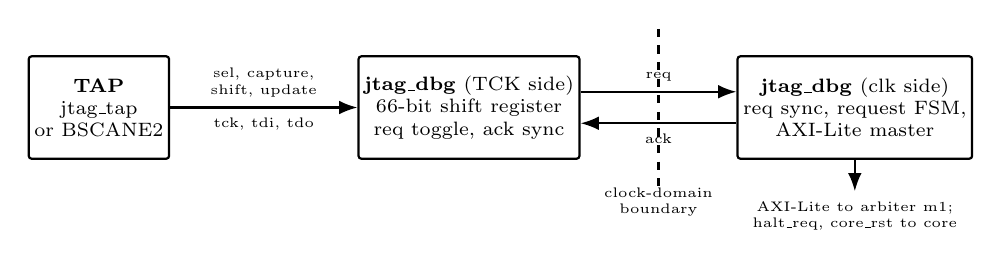
\begin{tikzpicture}[font=\scriptsize,>=Latex,thick,
  blk/.style={draw,rounded corners=1pt,inner sep=2pt,align=center,minimum height=13mm}]
  \node[blk,minimum width=17mm] (tap) at (0,0) {\textbf{TAP}\\jtag\_tap\\or BSCANE2};
  \node[blk,minimum width=24mm] (dr) at (4.7,0) {\textbf{jtag\_dbg} (TCK side)\\66-bit shift register\\req toggle, ack sync};
  \node[blk,minimum width=24mm] (fsm) at (9.6,0) {\textbf{jtag\_dbg} (clk side)\\req sync, request FSM,\\AXI-Lite master};
  \draw[->] (tap) -- node[above,font=\tiny,align=center]{sel, capture,\\shift, update} node[below,font=\tiny]{tck, tdi, tdo} (dr);
  \draw[->] ($(dr.east)+(0,2mm)$) -- node[above,font=\tiny]{req} ($(fsm.west)+(0,2mm)$);
  \draw[<-] ($(dr.east)+(0,-2mm)$) -- node[below,font=\tiny]{ack} ($(fsm.west)+(0,-2mm)$);
  \draw[dashed] ($(dr.east)!0.5!(fsm.west)+(0,10mm)$) -- ($(dr.east)!0.5!(fsm.west)+(0,-10mm)$);
  \node[font=\tiny,align=center] at ($(dr.east)!0.5!(fsm.west)+(0,-12mm)$) {clock-domain\\boundary};
  \draw[->] (fsm.south) -- ++(0,-4mm) node[below,font=\tiny,align=center]{AXI-Lite to arbiter m1;\\halt\_req, core\_rst to core};
\end{tikzpicture}}
\caption{Structure of the debug port. The two right-hand blocks form \reg{jtag\_dbg}; the request and acknowledge toggles are the only signals that cross between the \reg{TCK} and \reg{clk} domains.}
\label{fig:jtag}
\end{figure}

\subsection{Data Register Protocol}
The debug data register is 66 bits and is shifted least-significant bit
first (Table~\ref{tab:dr}). The host shifts in an operation, a data word and
an address; the request is issued on \emph{Update-DR}. Each subsequent scan
captures the response: bit~0 is \reg{busy}, bits [33:2] carry the data
returned by the last completed read, and bits [36:34] report the core
status. The host polls with \reg{op=nop} until \reg{busy} clears. A load
therefore costs two to three 66-bit scans per word; at a 10~MHz \reg{TCK}
the 1.5~KB \reg{hello} program loads in about 8~ms.

\begin{table}[t]
\caption{Debug data register (66 bits, LSB first)}
\label{tab:dr}
\centering
\footnotesize
\begin{tabular}{@{}lp{3.4cm}p{2.7cm}@{}}
\toprule
Bits & Shift in (host $\rightarrow$ SoC) & Shift out (SoC $\rightarrow$ host) \\
\midrule
{[1:0]}   & op: 0 nop, 1 read, 2 write, 3 control & bit 0 busy, bit 1 zero \\
{[33:2]} & data; for control: bit 0 halt, bit 1 core reset & last read data \\
{[34]}  & \multirow{3}{3.3cm}{address [31:0] (bits [65:34])} & halted \\
{[35]}  &  & halt request asserted \\
{[36]}  &  & core reset asserted \\
{[65:37]} & & zero \\
\bottomrule
\end{tabular}
\end{table}

\subsection{Clock-Domain Crossing}
\reg{TCK} and \reg{clk} are unrelated. On \emph{Update-DR} the TCK-domain
logic copies the request fields into holding registers and inverts a
request toggle. A three-flip-flop synchroniser in the \reg{clk} domain
detects the toggle edge (the first two flops synchronise, the third
provides the edge), at which point the holding registers have been stable
for at least two \reg{clk} periods and are read safely. When the transaction
completes the \reg{clk} domain inverts an acknowledge toggle, which is
synchronised back into the TCK domain by two flops; \reg{busy} is the
exclusive-or of the two toggles. The response payload (\reg{rdata},
\reg{halted}) is only sampled by the TCK side after \reg{busy} has cleared,
so it too is stable when read. Both synchronisers carry the \reg{ASYNC\_REG}
attribute; in the constraints \reg{TCK} is declared as a clock (30~MHz,
above the hardware manager's 15~MHz default) and placed in an asynchronous
clock group with the SoC clock.

\subsection{Bus Master and Core Control}
The \reg{clk}-domain state machine performs one AXI-Lite read or write per
request with the same registered-output discipline as the core, or, for a
control request, updates \reg{dbg\_halt\_req} and \reg{dbg\_core\_rst}. The
usual sequence to load and run a program is: halt; write the image
word-by-word; optionally read it back; assert and release core reset with
halt still asserted (the core restarts at address~0 but does not fetch); then
release halt.

\subsection{Host Side}
\reg{fpga/jtag\_host.tcl} drives the port from the Vivado hardware manager
with the raw \reg{scan\_ir\_hw\_jtag} and \reg{scan\_dr\_hw\_jtag} commands.
The instruction-register length (12 bits) and the \reg{USER1} opcode
(\reg{0x902}) are taken from the XCZU7EV boundary-scan description file
shipped with Vivado. The script provides \reg{dbg\_halt}, \reg{dbg\_run},
\reg{dbg\_reset}, \reg{dbg\_peek}, \reg{dbg\_poke} and \reg{dbg\_load}.

% =====================================================================
\section{Software Stack}\label{sec:sw}
% =====================================================================
The SoC runs C compiled by the unmodified xPack GNU tool-chain
(\reg{riscv-none-elf-gcc} 15.2) with \reg{-march=rv32i\_zicsr\_zifencei
-mabi=ilp32}. Four small pieces of code bridge the compiler and the
hardware.

\textbf{Linker script.} One 32~KB region at address 0 holds \reg{.text}
(with the start-up section placed first, at the reset vector), \reg{.rodata},
\reg{.data} and \reg{.bss}; the stack grows down from the top. Because the
whole image is loaded into the BRAM, \reg{.data} needs no copy at start-up.
An assertion fails the link if code, data and a 2~KB stack do not fit.

\textbf{Start-up code.} \reg{crt0.S} sets the global and stack pointers,
writes the trap vector into \reg{mtvec}, zeroes \reg{.bss}, calls
\reg{main} and parks in a loop if it returns.

\textbf{Trap vector.} \reg{trap.S} saves the sixteen caller-saved registers
on the stack, calls the C function \reg{trap\_handler(mcause, mepc)},
writes its return value back to \reg{mepc} (\reg{mepc+4} for \reg{ecall} and
\reg{ebreak}, unchanged for an interrupt), restores the registers and
executes \reg{mret}. A weak default handler reports the cause on the UART
and halts; programs override it.

\textbf{Board-support library.} \reg{soc.h} defines the memory map, register
bits and CSR access macros; \reg{uart.c} and \reg{timer.c} provide polled
character output and input, decimal and hexadecimal printing, and delays.

\textbf{Build flow.} A shared \reg{rules.mk} gives every program three
targets: \reg{make} builds the ELF, a raw binary, the \reg{\$readmemh} image
and a disassembly listing; \reg{make sim} rebuilds with \reg{-DSIM\_BUILD}
(short delays, self-terminating) and runs it in the simulator with the UART
output shown on the console; \reg{make install} copies the image into
\reg{rtl/program.hex} for the next bitstream. The ELF-to-image conversion is
a 15-line Python script.

\textbf{Programs.} \reg{hello} (1\,477~bytes) prints a banner and the memory
map, walks a pattern across the LEDs paced by the timer, reports the
switches whenever they change and echoes received characters.
\reg{irq\_demo} (1\,325~bytes) issues an \reg{ecall}, then enables the timer
interrupt and prints the tick count, \reg{mcycle} and \reg{minstret} from
the main loop while the interrupt service routine acknowledges the timer and
toggles an LED. Built with \reg{-DSIM\_BUILD}, each program writes a
completion code to the GPIO output that the testbench recognises, so both
double as regression tests.

% =====================================================================
\section{Verification}\label{sec:verif}
% =====================================================================
Verification proceeds from the instruction set upward to the routed netlist.
All simulations use the Vivado simulator (xsim); every step is scripted and
reproducible from the repository.

\subsection{Instruction-Set Regression}
The official \reg{riscv-tests} rv32ui suite \cite{riscv-tests} is vendored.
Its stock environment relies on CSRs and trap paths (\reg{tohost},
misaligned traps) that a minimal core does not have, so a 40-line
\reg{riscv\_test.h} was written that reports PASS by writing
\reg{0x0000600D} to the GPIO output and FAIL by writing
\reg{0xBAD00000}\,$|$\,test number, together with a linker script that places
each test at address~0. The runner \reg{run\_isa.py} compiles each program,
converts it to an image, simulates it under the generic testbench
\reg{tb\_isa.v} and tabulates the results; the whole suite takes about two
minutes. All 41 applicable tests pass (Table~\ref{tab:isa}); \reg{ma\_data}
is excluded because it requires misaligned-access traps. The harness was
checked for sensitivity by replacing the ALU's subtraction with addition:
\reg{sub} then fails at its third sub-test while every other test is
unaffected.

\begin{table}[t]
\caption{riscv-tests rv32ui results (cycles to PASS, RTL simulation)}
\label{tab:isa}
\centering
\scriptsize
\setlength{\tabcolsep}{3pt}
\begin{tabular}{@{}lr|lr|lr|lr@{}}
\toprule
add & 2147 & bltu & 1402 & lui & 147 & sltiu & 1007 \\
addi & 1032 & bne & 1277 & lw & 1189 & sltu & 2117 \\
and & 2247 & fence\_i & 1250 & or & 2262 & sra & 2382 \\
andi & 812 & jal & 97 & ori & 847 & srai & 1102 \\
auipc & 117 & jalr & 397 & sb & 2119 & srl & 2352 \\
beq & 1277 & lb & 1039 & sh & 2384 & srli & 1072 \\
bge & 1367 & lbu & 1039 & simple & 27 & st\_ld & 2286 \\
bgeu & 1492 & ld\_st & 5795 & sll & 2287 & sub & 2107 \\
blt & 1277 & lh & 1119 & slli & 1027 & sw & 2421 \\
 & & lhu & 1164 & slt & 2117 & xor & 2257 \\
 & & & & slti & 1007 & xori & 857 \\
\midrule
\multicolumn{8}{c}{41 / 41 PASS} \\
\bottomrule
\end{tabular}
\end{table}

\subsection{Generic Program Testbench}
\reg{tb\_isa.v} loads any image into the BRAM array, decodes the SoC's UART
transmit line and prints it on the console, optionally injects characters
into the receive line once the transmitter has been quiet for 50~$\mu$s (so
the stimulus lands after any banner), and stops on the PASS/FAIL code or a
watchdog. The same testbench runs the ISA suite and the application
programs.

\subsection{Application Programs}
\reg{hello} passes with the full banner, the switch report, the echo of the
injected characters and the completion code; \reg{irq\_demo} passes with the
\reg{ecall} acknowledged and three timer interrupts serviced, each tick
printed with the cycle and instruction counters.

\subsection{Debug Port}
\reg{tb\_jtag.v} contains a JTAG bus-functional model that drives real
\reg{TMS}/\reg{TDI} sequences into \reg{jtag\_tap}. With the BRAM initially
holding only \reg{jal x0,0}, it reads \reg{IDCODE}, halts the core and checks
the halted flag, writes the 382-word \reg{hello} image through the debug
master and reads every word back, resets and releases the core, then, while
the program runs and prints, reads \reg{GPIO\_IN} and \reg{TIMER\_COUNT}
over JTAG (which also exercises the arbiter under contention), and finally
waits for the program's completion code. The test passes in 1.43~M clock
cycles of simulation.

\subsection{Post-Implementation Simulation}
After place and route, \reg{write\_verilog -mode funcsim} produces the
gate-level netlist of \reg{zcu104\_top}, including the block RAMs with their
initialisation strings and the \reg{BSCANE2}. A board-level testbench drives
the real 300~MHz differential clock, leaves the reset button released (so the
wrapper's 128-cycle self-reset is what starts the SoC), decodes the UART at
115\,200~baud and passes when the banner begins to appear. The routed netlist
prints \reg{Hello} at $t = 610\,\mu$s; the simulation takes about 35~s.

% =====================================================================
\section{FPGA Implementation}\label{sec:impl}
% =====================================================================
\subsection{Board Wrapper and Constraints}
\reg{zcu104\_top} adds to \reg{soc\_top} an \reg{IBUFDS} for the 300~MHz
DDR4-bank oscillator, a \reg{BUFGCE\_DIV} dividing by three, a two-flop
synchroniser and 128-cycle stretcher on the \reg{CPU\_RESET} button, the
\reg{BSCANE2} with a \reg{BUFG} on its \reg{TCK}, and the pin mapping of
Table~\ref{tab:pins}. Pin locations and I/O standards are taken from the
ZCU104 board file shipped with Vivado. The constraints define the 300~MHz
input clock (the 100~MHz clock is derived automatically), the 30~MHz
\reg{TCK} clock in an asynchronous group, and false paths on the switch,
button, LED and UART pins, which have no timing requirement.

\begin{table}[t]
\caption{ZCU104 pin assignment}
\label{tab:pins}
\centering
\footnotesize
\begin{tabular}{@{}p{3.3cm}p{2.5cm}l@{}}
\toprule
Signal & Package pins & I/O standard \\
\midrule
\reg{clk300\_p/n} & AH18 / AH17 & DIFF\_SSTL12 \\
\reg{cpu\_reset} (active high) & M11 & LVCMOS33 \\
\reg{dip[3:0]} & E4, D4, F5, F4 & LVCMOS33 \\
\reg{pb[3:0]} & B4, C4, B3, C3 & LVCMOS33 \\
\reg{led[3:0]} & D5, D6, A5, B5 & LVCMOS33 \\
\reg{uart\_tx} / \reg{uart\_rx} (CP2108 PL channel) & C19 / A20 & LVCMOS18 \\
JTAG & device TAP via \reg{BSCANE2} & -- \\
\bottomrule
\end{tabular}
\end{table}

\subsection{Flow}
A non-project Tcl script runs \reg{synth\_design}, \reg{opt\_design},
\reg{place\_design}, \reg{phys\_opt\_design}, \reg{route\_design} and
\reg{write\_bitstream} with default directives and writes the utilisation,
timing, power and DRC reports. A second script regenerates the Vivado GUI
project from the same sources for interactive work. The flow takes about 25
minutes on an 8~GB laptop, dominated by placement.

\subsection{Results}
Table~\ref{tab:util} gives the utilisation by block and
Table~\ref{tab:timing} the timing summary. All constraints are met. The
worst setup path on the 100~MHz clock leaves 5.3~ns of the 10~ns period
unused, so the design would close at about 200~MHz without modification;
100~MHz was kept so that the UART divisor and the timer values remain round
numbers. The critical path (4.55~ns, 9 logic levels, 77\,\% routing) runs from
the instruction register through the register-file read (\reg{funct3}
selects the branch condition, \reg{rs1}/\reg{rs2} address the LUT-RAM),
the branch comparator and the next-PC multiplexer to \reg{pc\_reg}, as
expected for a multicycle core that resolves branches combinationally in
the same state that decodes them.

The whole SoC uses 0.74\,\% of the device's look-up tables and 2.6\,\% of
its block RAM. The JTAG debug port (debug register, synchronisers, bus
master, arbiter and the core's halt hook) costs about 190 look-up tables and
230 flip-flops, about 11\,\% of the SoC, and left the SoC clock's slack
essentially unchanged (from $+5.36$ to $+5.28$~ns). The vectorless power
estimate is 0.631~W, of which only 0.017~W is dynamic: the design is far too
small to move the device's static floor.

\begin{table}[t]
\caption{Utilisation on the XCZU7EV after place and route}
\label{tab:util}
\centering
\scriptsize
\setlength{\tabcolsep}{3pt}
\resizebox{\columnwidth}{!}{%
\begin{tabular}{@{}llrrrrr@{}}
\toprule
Instance & Module & LUTs & LUTRAM & FFs & RAMB36 & DSP \\
\midrule
\reg{zcu104\_top} & wrapper + SoC & 1\,717 & 40 & 995 & 8 & 0 \\
\reg{u\_soc} & \reg{soc\_top} & 1\,710 & 40 & 985 & 8 & 0 \\
\reg{u\_core} & \reg{riscv\_core} & 1\,400 & 40 & 488 & 0 & 0 \\
\reg{u\_dbg} & \reg{jtag\_dbg} & 164 & 0 & 228 & 0 & 0 \\
\reg{u\_uart} & UART + tx + rx & 73 & 0 & 87 & 0 & 0 \\
\reg{u\_timer} & timer & 66 & 0 & 103 & 0 & 0 \\
\reg{u\_gpio} & GPIO & 1 & 0 & 72 & 0 & 0 \\
-- & BRAM ctrl, arbiter, xbar & $\approx 6$ & 0 & $\approx 7$ & 8 & 0 \\
\bottomrule
\end{tabular}}
\end{table}

\begin{table}[t]
\caption{Timing summary (setup/hold/pulse-width slack)}
\label{tab:timing}
\centering
\scriptsize
\setlength{\tabcolsep}{3pt}
\resizebox{\columnwidth}{!}{%
\begin{tabular}{@{}lrrrrr@{}}
\toprule
Clock & Period (ns) & Endpoints & WNS (ns) & WHS (ns) & WPWS (ns) \\
\midrule
\reg{clk} (SoC) & 10.0 & 2\,370 & $+5.275$ & $+0.003$ & $+2.791$ \\
\reg{jtag\_tck} & 33.3 & 165 & $+31.228$ & $+0.017$ & $+16.391$ \\
\reg{clk300} (input) & 3.33 & 1 & -- & -- & $+2.262$ \\
\bottomrule
\end{tabular}}
\end{table}

% =====================================================================
\section{Problems Encountered and Design Lessons}\label{sec:lessons}
% =====================================================================
The following problems arose during the project; each changed either the
design or the methodology.

\textbf{A hand-assembled instruction.} The first test program stored its
result to address \reg{0xF} instead of the GPIO register and the LED never
changed. A cycle-by-cycle trace showed the core computing exactly what it was
told: the store had been hand-encoded with \reg{rs1=x3} instead of
\reg{x4}. The lesson is that programs must come from an assembler and that
a regression must be independent of the program under test; both led to the
\reg{riscv-tests} flow.

\textbf{Simulation-only initialisation.} The BRAM's \reg{\$readmemh} was
originally inside a \reg{translate\_off} region, so the bitstream would have
contained an empty program memory. Making the initialisation synthesisable,
and moving the memory array into a reset-free clocked block so that block RAM
is inferred rather than 8\,192 words of distributed RAM, fixed both the
function and the area.

\textbf{Timescale and reset discipline.} The design files carried no
\reg{`timescale}; the GUI hid the resulting elaboration error with
\reg{--relax}. Twenty-three registers were assigned in asynchronous-reset
blocks without a reset value and produced synthesis warnings. Both were
corrected, and the standalone simulation flow deliberately elaborates without
\reg{--relax} so that such issues are visible.

\textbf{Vendor batch wrappers.} The Vivado \reg{.bat} wrappers on Windows
split arguments at ``\reg{=}'', so simulator plus-arguments cannot carry a
path. The testbenches therefore read their image from a fixed file name and
their watchdog value from a small text file, which is also simpler to script.

\textbf{Single-byte UART receiver.} Characters injected while the program
was still printing its banner were overwritten in the receiver's one-byte
register. Rather than hide this with a magic delay, the testbench waits for
the transmit line to be idle before injecting, and the limitation is
documented for software.

\textbf{TDO sampling race.} The first JTAG testbench sampled \reg{TDO} in the
same time step as the falling \reg{TCK} edge that updates it and read every
word shifted by one bit. Sampling a quarter period after the edge removed the
race; the RTL was unchanged.

\textbf{Unconstrained JTAG clock.} The first build with \reg{BSCANE2} had no
clock defined on its \reg{TCK}, so the debug register's paths would have
been unconstrained, silently. A clock constraint and an asynchronous clock
group were added before the results were recorded.

% =====================================================================
\section{Conclusion and Future Work}\label{sec:conclusion}
% =====================================================================
\soc\ demonstrates a complete, from-scratch SoC whose every block is
understood and tested: an RV32I core with machine-mode traps and interrupts
that passes the official instruction-set suite, an AXI4-Lite fabric with two
masters, four peripherals, a JTAG debug port that loads and controls
programs through the FPGA's own test-access port, and a C tool-chain. The
placed-and-routed design occupies 1\,710 LUTs and 8 block RAMs on the
XCZU7EV, meets timing at 100~MHz with 5.3~ns to spare, and its netlist boots
and prints in gate-level simulation.

Three extensions are natural next steps. An illegal-instruction exception
and misaligned-access traps would complete the M-mode exception model and
allow the remaining \reg{riscv-tests} programs to run. A two- or three-stage
pipeline would raise the throughput from 5--7 cycles per instruction towards
one, at the cost of hazard logic that the existing regression is well placed
to verify. And extending the debug port to the RISC-V External Debug
Specification (a debug module with abstract commands and a debug-mode CSR
set) would let \reg{gdb} attach through OpenOCD, building on the halt, reset
and memory-access mechanisms already in place.

% =====================================================================
\begin{thebibliography}{9}
\bibitem{riscv-unpriv} A. Waterman and K. Asanovi\'c, Eds., \emph{The RISC-V
Instruction Set Manual, Volume I: Unprivileged ISA}, Document Version
20191213, RISC-V Foundation, Dec. 2019.

\bibitem{riscv-priv} A. Waterman, K. Asanovi\'c, and J. Hauser, Eds.,
\emph{The RISC-V Instruction Set Manual, Volume II: Privileged
Architecture}, Document Version 20211203, RISC-V International, Dec. 2021.

\bibitem{axi} Arm Ltd., \emph{AMBA AXI and ACE Protocol Specification},
IHI 0022, 2021, ch.~B ``AMBA AXI4-Lite''.

\bibitem{ieee1149} \emph{IEEE Standard for Test Access Port and Boundary-Scan
Architecture}, IEEE Std 1149.1-2013, 2013.

\bibitem{ug974} Xilinx Inc., \emph{UltraScale Architecture Libraries Guide},
UG974, 2025 (``BSCANE2'', ``BUFGCE\_DIV'').

\bibitem{ug1267} Xilinx Inc., \emph{ZCU104 Evaluation Board User Guide},
UG1267, v1.1, 2018.

\bibitem{riscv-tests} RISC-V Software Collaboration, ``riscv-tests,''
\url{https://github.com/riscv-software-src/riscv-tests}, commit 2ebecad,
Aug. 2026.

\bibitem{ug900} Xilinx Inc., \emph{Vivado Design Suite User Guide: Logic
Simulation}, UG900, 2025.

\bibitem{ug908} Xilinx Inc., \emph{Vivado Design Suite User Guide:
Programming and Debugging}, UG908, 2025 (hardware-manager JTAG Tcl commands).
\end{thebibliography}

\end{document}
